
\begin{subsubsection}{KDA on parabolic data}
Another data set is shown in Figure \ref{fig:parab_data}. Again, this is easily separable, but it's clear that the separation is nonlinear. Again, for LDA, we obtain the failed classification (Figure \ref{fig:LDA_parab}) and the successful classification in Figure \ref{fig:KDA_proj_parab}.
\\
\begin{minipage}{1.0\textwidth}
    \begin{figure}[H]
    \centering
    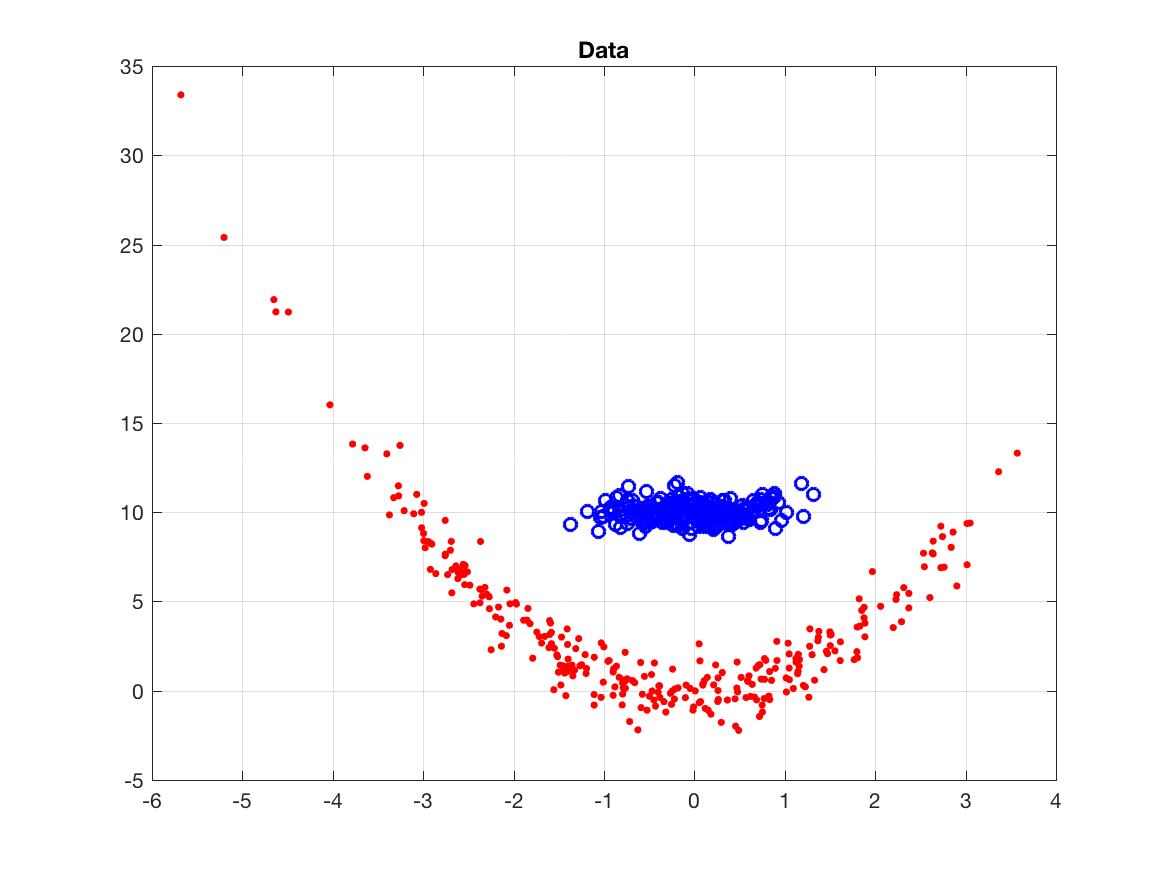
\includegraphics[trim={0cm 0cm 0cm 0cm},clip,width=0.8\columnwidth]{kda_test/parab_data}
    \caption{Parabolically-separable data}
    \label{fig:parab_data}
    \end{figure}
\end{minipage}

\centerline{\begin{minipage}{0.6\textwidth}
    \begin{figure}[H]
    \centering
    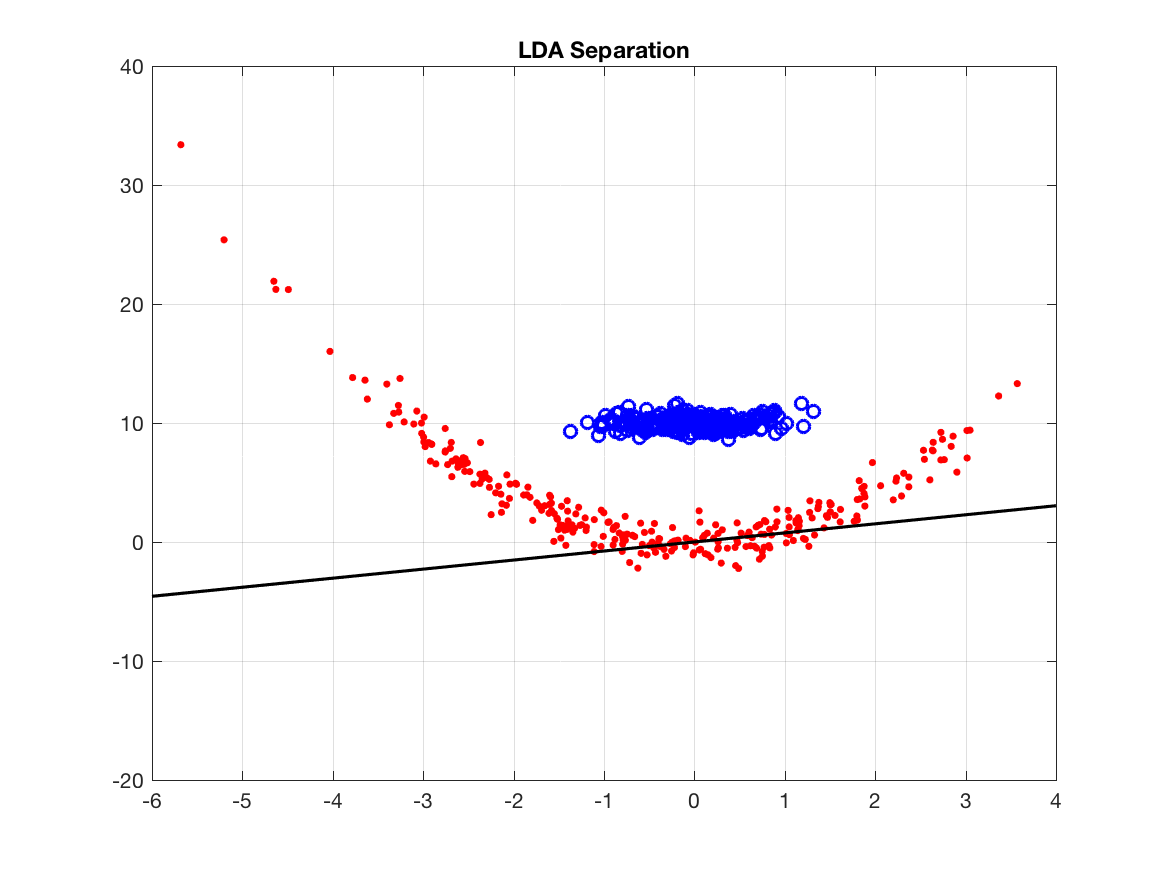
\includegraphics[trim={0cm 0cm 0cm 0cm},clip,width=1.0\columnwidth]{kda_test/LDA_parab}
    \caption{Figure \ref{fig:parab_data} data with LDA projection vector}
    \label{fig:LDA_parab}
    \end{figure}
\end{minipage}}

\centerline{\begin{minipage}{0.6\textwidth}
    \begin{figure}[H]
    \centering
    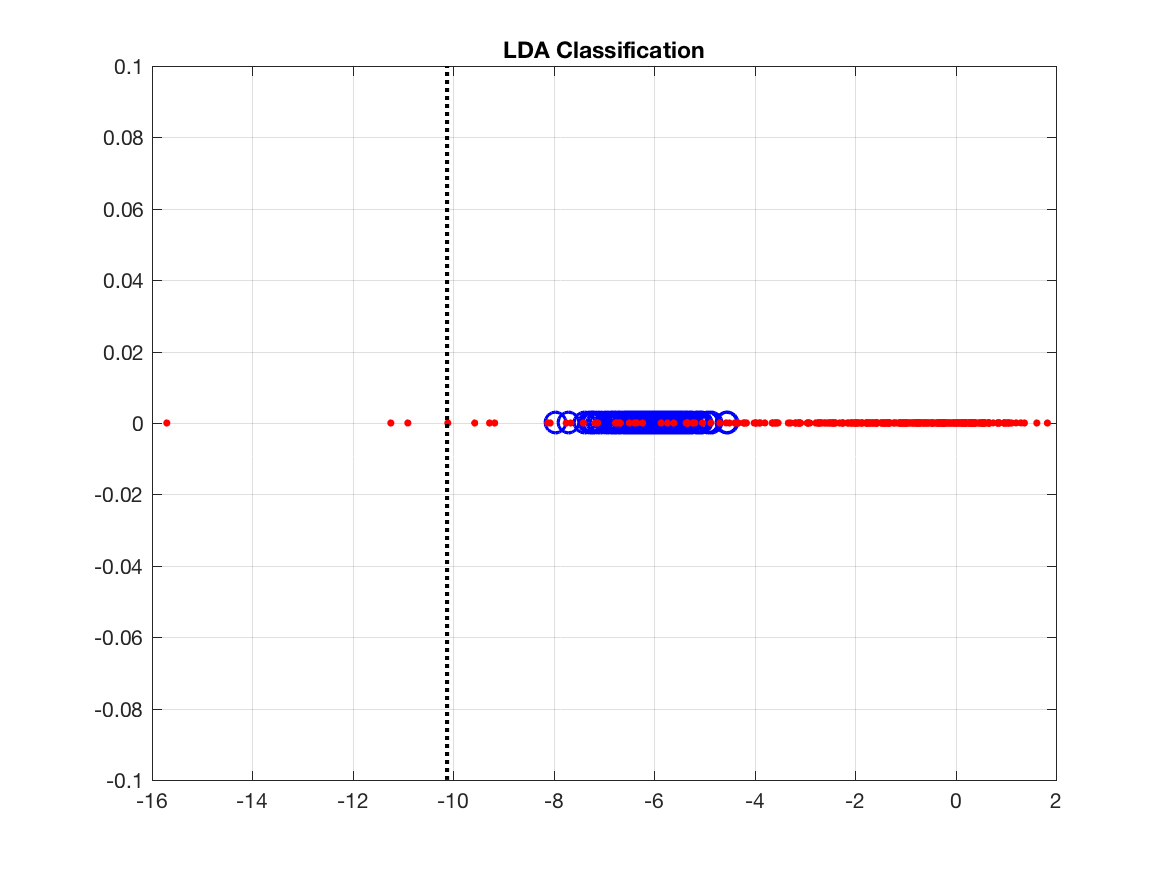
\includegraphics[trim={0cm 0cm 0cm 0cm},clip,width=1.0\columnwidth]{kda_test/LDA_proj_parab}
    \caption{Figure \ref{fig:parab_data} LDA classification}
    \label{fig:LDA_proj_parab}
    \end{figure}
\end{minipage}}

\centerline{\begin{minipage}{0.8\textwidth}
    \begin{figure}[H]
    \centering
    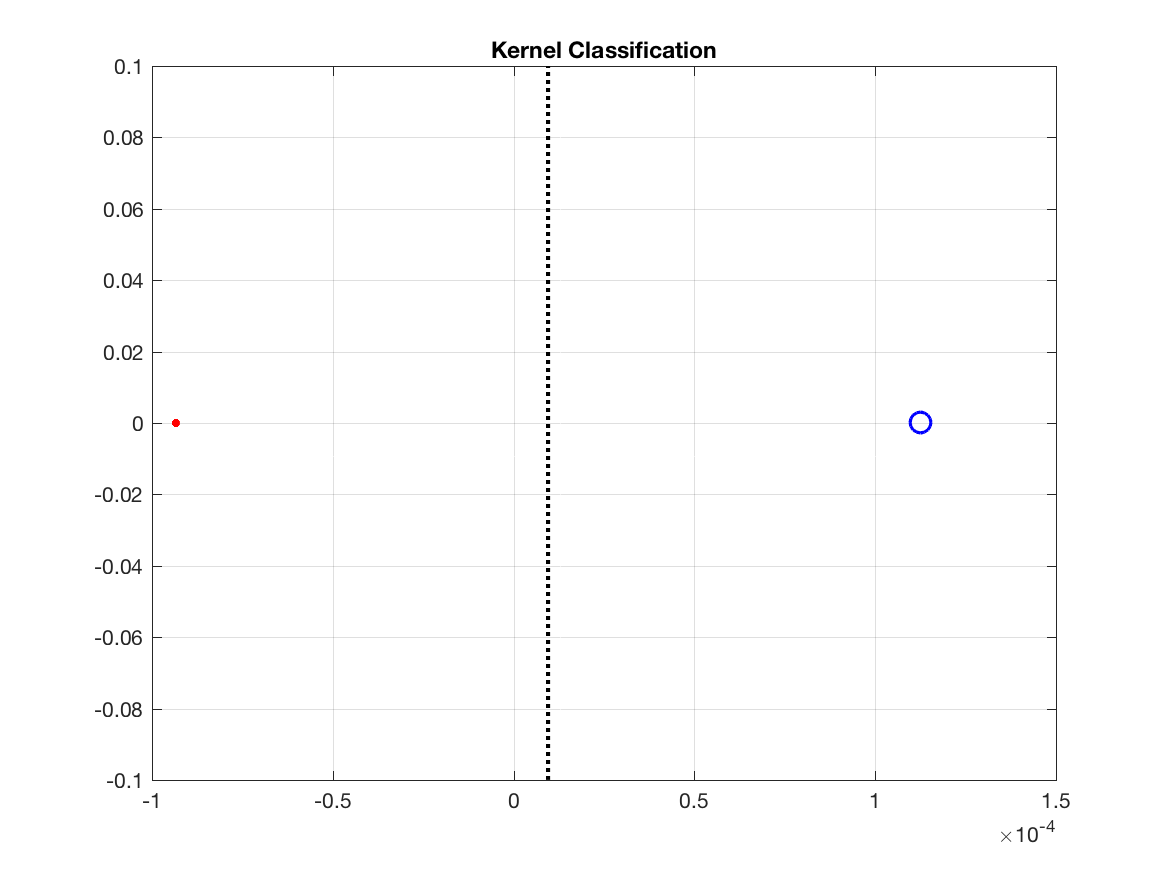
\includegraphics[trim={0cm 0cm 0cm 0cm},clip,width=0.8\columnwidth]{kda_test/KDA_proj_parab}
    \caption{Figure \ref{fig:parab_data} KDA classification}
    \label{fig:KDA_proj_parab}
    \end{figure}
\end{minipage}}
\end{subsubsection}
